\section{Linear Regression}
\smallskip \hrule height 2pt \smallskip

\underline{Ordinary Least Squares} \hfill \\

Notation:
\begin{itemize}
	\item \textbf{$x_i$}: an input data point.  \_\_ rows by \_\_ columns. 
	\item \textbf{$y_i$}: a predicted output
	\item \textbf{$\widehat{y_i}$}: a predicted output
	\item \textbf{$\widehat{y}$}: 
	\item \textbf{$w_k$}: weight k
	\item \textbf{$\bm{w}^*$}: the vector of weights found in regression.   
	\item \textbf{$f_k(x_i)$}
	\item \textbf{$t$}: what we want to regress against
	\item \textbf{$t_j$}: the output variable that you either have data for or are predicting. 
	\item \textbf{$t(\bm{x})$}: Data.  "Mapping from x to t(x)"
	\item \textbf{$H$}: $H = \{ h_1, \dots, h_K \}$.  Basis functions.  In the simplest case, they can just be the value of an input variable/feature or a constant (for bias).  
	\item \textbf{$L_2$}: The $L_2$.  Can appear as a loss function to describe the deviation from data or as a penalty.  
		% Erick clarification
	\item \textbf{$ || \widehat{w} ||_1$}: "$L_1$" penalty.  The "Manhattan distance".  Like traveling a, b in a pythagorean triangle.  $\sum |x_i|$
	\item \textbf{$ || \widehat{w} ||_2$}.  "$L_2$" penalty.  Euclidean length of a vector.  Like c in a pythagorean triangle.  $\sqrt{\sum |x_i|^2}$	
\end{itemize}

\underline{Vocab}:
\begin{itemize}
	\item \textbf {bias-variance tradeoff} - the problem of simultaneously minimizing two sources of error that prevent 
			supervised learning algorithms from generalizing beyond their training set.  % https://en.wikipedia.org/wiki/Bias%E2%80%93variance_tradeoff
			\begin{itemize}  
				\item The bias is error from erroneous assumptions in the learning algorithm. 
					High bias can cause an algorithm to miss the relevant relations between features 
					and target outputs (underfitting).
				\item The variance is error from sensitivity to small fluctuations in the training set. 
					High variance can cause overfitting: modeling the random noise in the training 
					data, rather than the intended outputs.
			\end{itemize}
	\item \textbf{basis function}
	\item \textbf{bias} (parameter): like the intercept in a linear equation.  The part that doesn't depend on the features. 
	\item \textbf{bias} (learning bias):  (?? "inductive bias" ??)  - 
	\item \textbf{hyperplane} - a plane, usually with more than 2 dimensions. 
	\item \textbf{input variable} - a.k.a. feature.  % https://en.wikipedia.org/wiki/Dependent_and_independent_variables
		E.g. a column like CEO salary for rows of data corresponding to different companies.
	\item \textbf{response variable} - synonyms: "dependent variable", "regressand", "predicted variable", "measured variable", "explained variable", "experimental variable", "responding variable", "outcome variable", and "output variable".   E.g. a predicted stock price.   
	\item \textbf{regularization} -  introducing additional information in order to solve an ill-posed problem or to prevent overfitting. 
	% https://en.wikipedia.org/wiki/Regularization_(mathematics)
	E.g. applying a penalty for large parameters in the model. 
	\item \textbf{ridge regression} - 
	\item \textbf{vector norm}: put in a vector and get out a number like length or size.  Real valued function of some sort of vector or matrix quantity. 
	\item \textbf{hyperparameters}: \hfill \\
	$\lambda$, not $w$.  Parameters that control your actual parameters.  \hfill \\ \hfill \\
	% Wrong?!?   Norm 1 and norm 2 are not "parameters".  $\dots$ model design.  \hfill \\
	% Wrong?!?   Different values of lambda won't change the complexity of the model.  \hfill \\

	% Erick definition:
	In Bayesian analysis, the parameters that don't touch the data.  
	Like the parameters for the prior on the prior.  
	Called the ridge regression $\lambda$ a hyperparameter, though this is a stretch in the terminology.  \hfill \\
	Class version: 
	\item \textbf{feature selection}: explicitly select features that can go into your model instead of throwing all features in. 
	\item \textbf{loss function}:  
		% wikipedia:
		 A function that maps an event or values of one or more variables onto a real number intuitively representing some 			"cost" associated with the event. 
		 An optimization problem seeks to minimize a loss function. \hfill \\
		% week 4 typed notes near bottom. 
		$\sum_j (t(x_j) - \sum w_i h(x_i))^2$. (least-squares error ($L_2$))  (??? = training error??)
	\item \textbf{training set error}:  *doesn't include the regularization penalty!*.  A.k.a. "training error".  
			Sum of squares error divided by the number of points.   See formula later. 
%	\item \textbf{training error}:  sononomous
\end{itemize}

\subsection{Ordinary Least Squares}
total error = $\displaystyle \sum_i (y_i-\hat{y_i})^2 = \sum_i(y_i - \sum_k w_k f_k(x_i))^2$ \hfill \\
$i$ is for each data point, $k$ is for each of the k basis functions. 

 \hfill \\ \hfill \\

Under the additional assumption that the errors be normally distributed, OLS is the maximum likelihood estimator. \hfill \\ % https://en.wikipedia.org/wiki/Ordinary_least_squares
?? Use words to describe what subset of regression in general this is.  What is ordinary? What are we limiting?  \hfill \\
 \hfill \\

The regression problem: \hfill \\
Given basis functions $\{ h_1, \dots, h_K \}$  with $h_i(\bf{x}) \in \mathbb{R}$,  \hfill \\
	find coefficients $\bm{w} = \{ w_1, \dots, w_k \}$.  \hfill \\%  
$t(\bm{x}) \approx \widehat{f}(\bm{x}) = \sum_i w_i h_i(\bm{x})$     \hfill \\  \hfill \\


This is called linear regression b/c it is linear in the parameters. 
We can still fit to nonlinear functions by using nonlinear basis functions;  $f_k \rightarrow  h_i$
Minimize the \textbf{residual squared error}: \hfill \\
$ \displaystyle \bm{w}* = \argmin_{\bm{w}}  \sum_j (t(\bm{x}_j) - \sum_i w_i h_i(\bm{x}_j))^2$  \hfill \\
$j$ for each data point, $i$ for the number of weights, which is the number of basis functions.  \hfill \\
\hfill \\  \hfill \\

For fitting a line in 2D space, your basis functions are $\{ h_1(x) = x, h_2(x) = 1 \}$.  $h_2(x)$ = 1 is the (constant) bias basis function.  The size of $w_2$ controls the effect in prediction.    \hfill \\  \hfill \\

To fit a parabola, your basis functions could be $\{ h_1(x) = x^2, h_2(x)=x, h_3(x)=1 \}$.   \hfill \\
Want a 2D parabola? Use $\{ h_1(x) = x_1^2, h_2(x)=x_2^2, h_3(x)=x_1 x_2, \dots \}$. \hfill \\
Can define any basis functions $h_i(\bm{x})$ for n-dimensional input $\bm{x} = <x_1, \dots, x_n>$
\hfill \\  \hfill \\

\underline{Linear in feature space vs linear in the parameter space}:  \hfill \\
When we want to fit a parabola, we are still using a function that is linear in \underline{parameter} space. 
The weight matrix is still all constants. 
When we use nonlinear basis functions, we are nonlinear in \underline{feature} space.  The basis functions may be transformations of the input parameters. 
 \hfill \\ \hfill \\

\subsection{Regression: matrix notation}
\begin{align*}
	\bm{w}* &= \argmin_w \sum_j(t(\bm{x}_j - \sum_i w_i h_i(\bm{x}_j))^2  \\
	\bm{w}* &= \argmin_w (\bm{Hw} -\bm{t})^T (\bm{Hw} -\bm{t})
\end{align*}
$  (\bm{Hw} -\bm{t})^T (\bm{Hw} -\bm{t})$ is the residual error.  
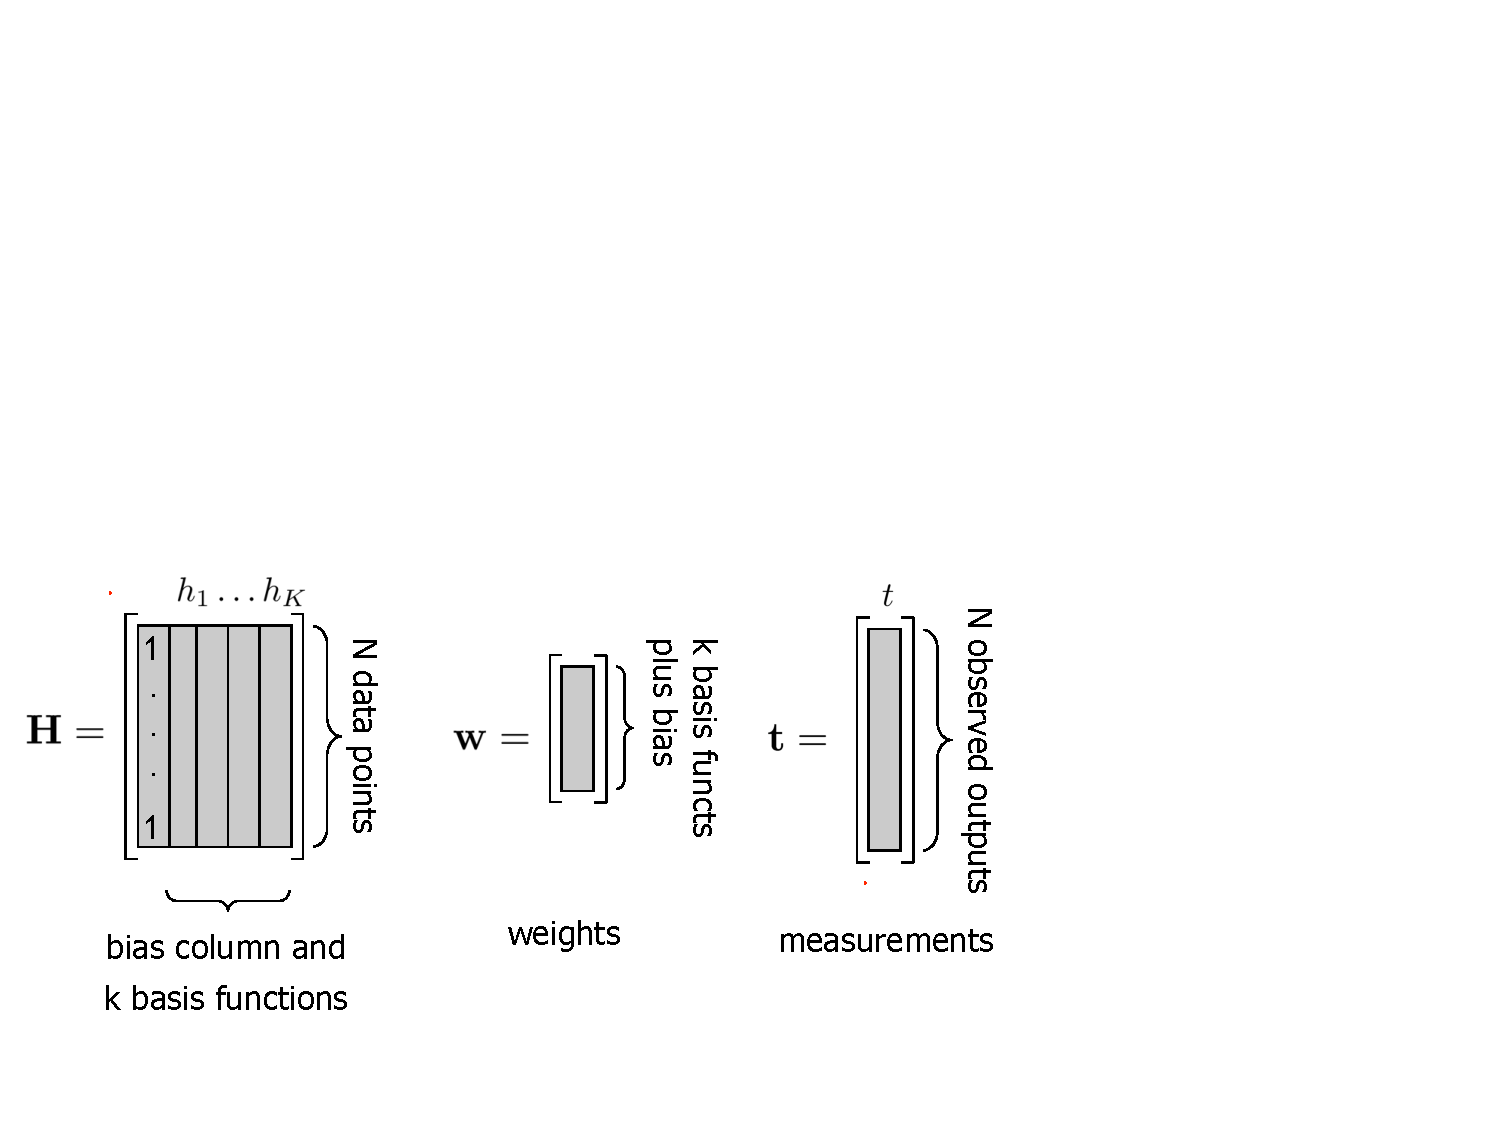
\includegraphics[width=3in]{figures/Least_squares_matricies.pdf}

\subsection{Regression: closed form solution}
 % derivation: http://courses.cs.washington.edu/courses/cse446/16wi/Slides/4_LinearRegression.pdf
\begin{align*}
	\bm{w}^* = \argmin_w (\bm{Hw} -\bm{t})^T (\bm{Hw} -\bm{t})  & \\
	\bm{F}(\bm{w}) =  \argmin_w (\bm{Hw} -\bm{t})^T (\bm{Hw} -\bm{t}) & \\
	\triangledown_{\bm{w}}\bm{F}(\bm{w}) = 0 \\
	2 \bm{H}^T (\bm{H}\bm{w}-\bm{t}) = 0  & \\
	(\bm{H}^T\bm{H}\bm{w}) - \bm{H}^T\bm{t} = 0 & \\
	\bm{w}^* = (\bm{H}^T\bm{H})^{-1}\bm{H}^T\bm{t} &
\end{align*}

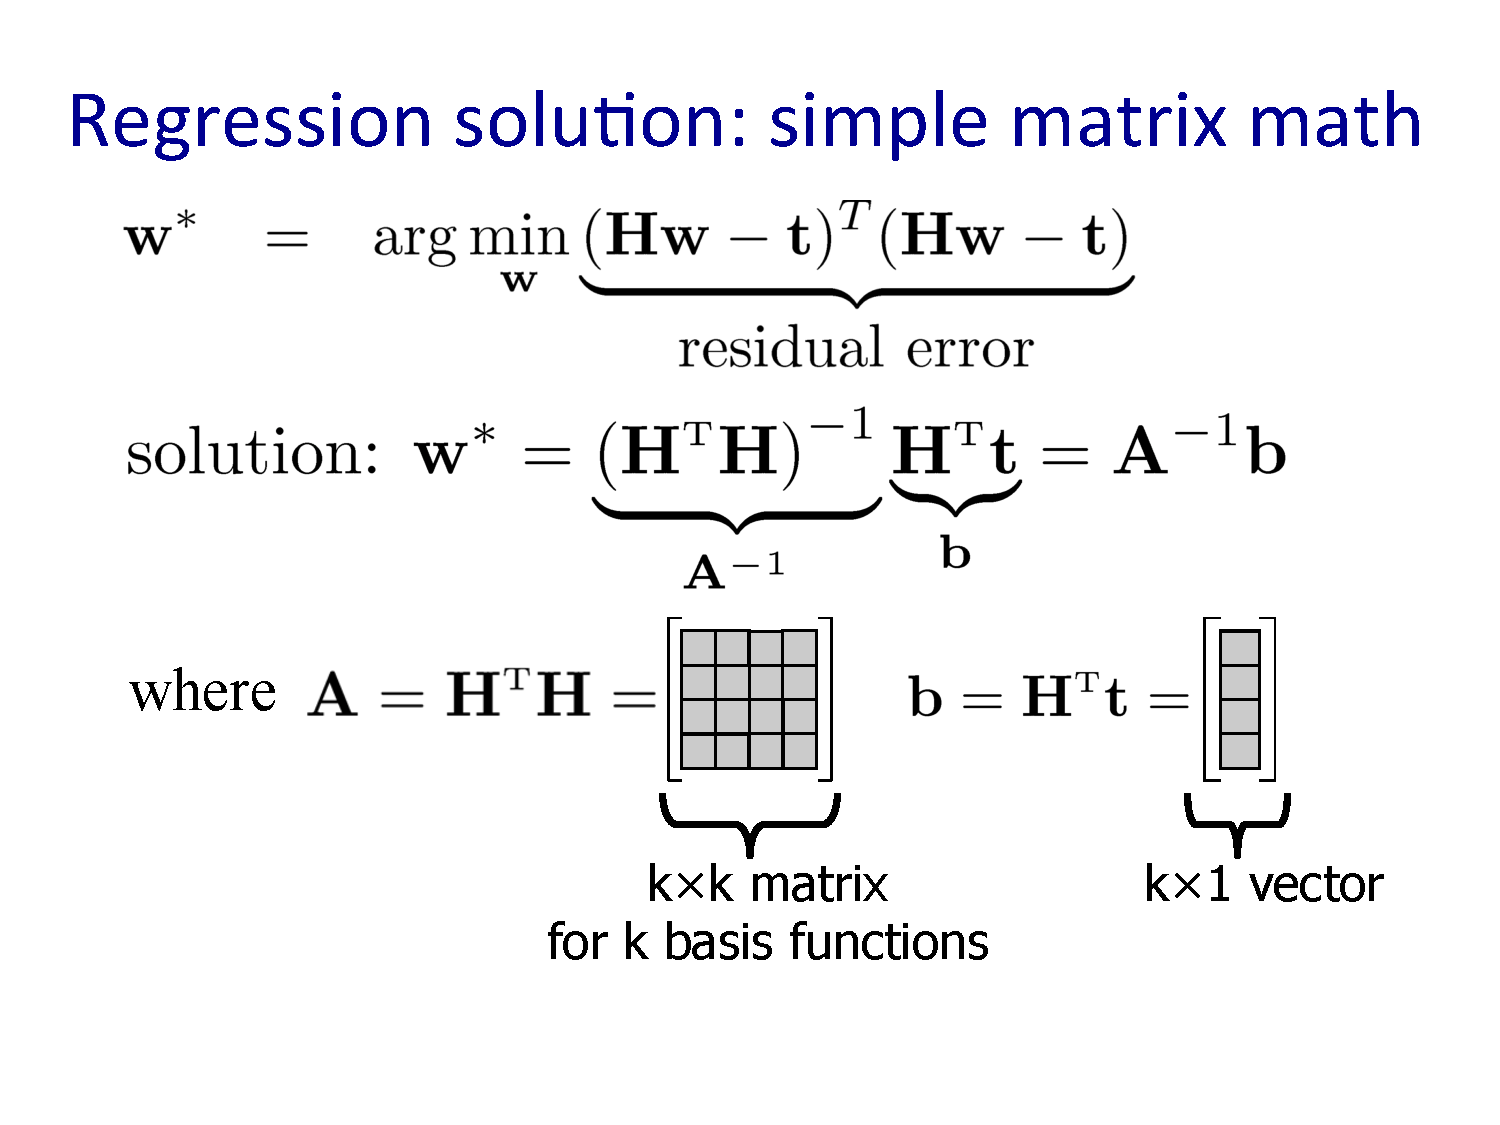
\includegraphics[width=3in]{figures/Regression_matrix_math.pdf}

Dimensions: 
\begin{itemize}
	\item $\bm{t}$:  N-dimensional  (N = \# of input data points) 
	\item $\bm{w}$: 
	\item $\bm{H}$: k + 1 by N.  N is \# of rows. 
\end{itemize}
\hfill \\

\subsubsection{Linear regression prediction is a linear function plus Gaussian noise}

If we assume that our data y_i is drawn from a linear function with some zero-mean Gaussian noise, i.e.

$$y_i = \sum_j w_j X_ij + \epsilon_i$$
(where $\episilon_i$ is zero-mean gaussian noise drawn from Normal(0, $\sigma$)

Then we can show that the MLE estimates of w_j are exactly the optimal weights obtained by minimizing the SSE: $\sum_i (y_i - w^T X_i)^2$

(note that the variance $\sigma$ actually doesn't matter for the derivation, you can just assume it's some positive number).

We can model as linear combination of basis functions + noise $\epsilon$.  
It's safe to assume epsilon comes from Gaussian distribution.  \hfill \\

$t(\bm{x}) = \sum_i w_i h_i(\bm{x}) + \epsilon $ \hfill \\
Note: no $\mu$ because we set it to zero.  \hfill \\

We can learn $\bf{w}$ using MLE: 
$P(t | x, w, \sigma) = \frac{1}{\sigma \sqrt{2 \pi}} e^\frac{-[t - \sum_i w_i h_i(x)]^2}{2 \sigma^2}$
Take the log and maximize with respect to w:  (maximizing log-likelihood with respect to w) \hfill \\
$\displaystyle \ln P(D | \bm{w}, \sigma) = \ln(\frac{1}{\sigma \sqrt{2 \pi}})^N \prod_{j=1}^N e^\frac{-[t_j - \sum_i w_i h_i(x_j)]^2}{2 \sigma^2}$ \hfill \\
Now find the w that maximizes this: \hfill \\
$\argmax_w \ln(\frac{1}{\sigma \sqrt{2 \pi}})^N + \sum_{j=1}^N \frac{-[t_j - \sum_i w_i h_i(x_j)]^2}{2 \sigma^2}$ \hfill \\
the first term isn't impacted by $w$ so  \hfill \\
$= \argmax_w  \sum_{j=1}^N \frac{-[t_j - \sum_i w_i h_i(x_j)]^2}{2 \sigma^2}$ \hfill \\
switch to $\argmin_w$ when we divide by -1.  The numerator is constant.:  \hfill \\
$= \argmin_w  [t_j - \sum_i w_i h_i(x_j)]^2 $ \hfill \\

\textbf{Least-squares Linear Regression is MLE for Gaussians!!!}  \hfill \\ \hfill \\

If you have a polynomial you are fitting, how many basis functions are there (??)  \hfill \\ % asked Wed 1/27


\subsection{OLS Protocol (incomplete)}  \hfill \\
\begin{enumerate}
	\item Chose your basis functions $h_i$.  (Requires expertise).  Can be nonlinear, e.g. $x_1^2, \sin(x)$, etc. 
		\begin {itemize}
			\item 
				The number of parameters is len(H) + 1 (bias).  
				E.g. for fitting a parabola (formula $y = ax^2 + bx + c$), 
				you have 3 parameters: weights for basis functions $x$, $x^2$, and bias. 
				Typically the \# of basis functions is $<$ the \# of features.
		\end {itemize}
	\item Chose a regularization method so your weights don't get too big.  (see below)
	\item Plug them in to regression to get the weights ($w_i$s).  (Form the sum (residual squared error + regularization) that you want to minimize, then minimize.)    
	\item Make sure your weights aren't too big. 
	
\end{enumerate}

\subsection{Regularization in Linear Regression}  \hfill \\
You need to regularize to prevent parameters from growing too large.  
Both of these were built from the same set of basis functions; the right one is clearly over-fit. \hfill \\
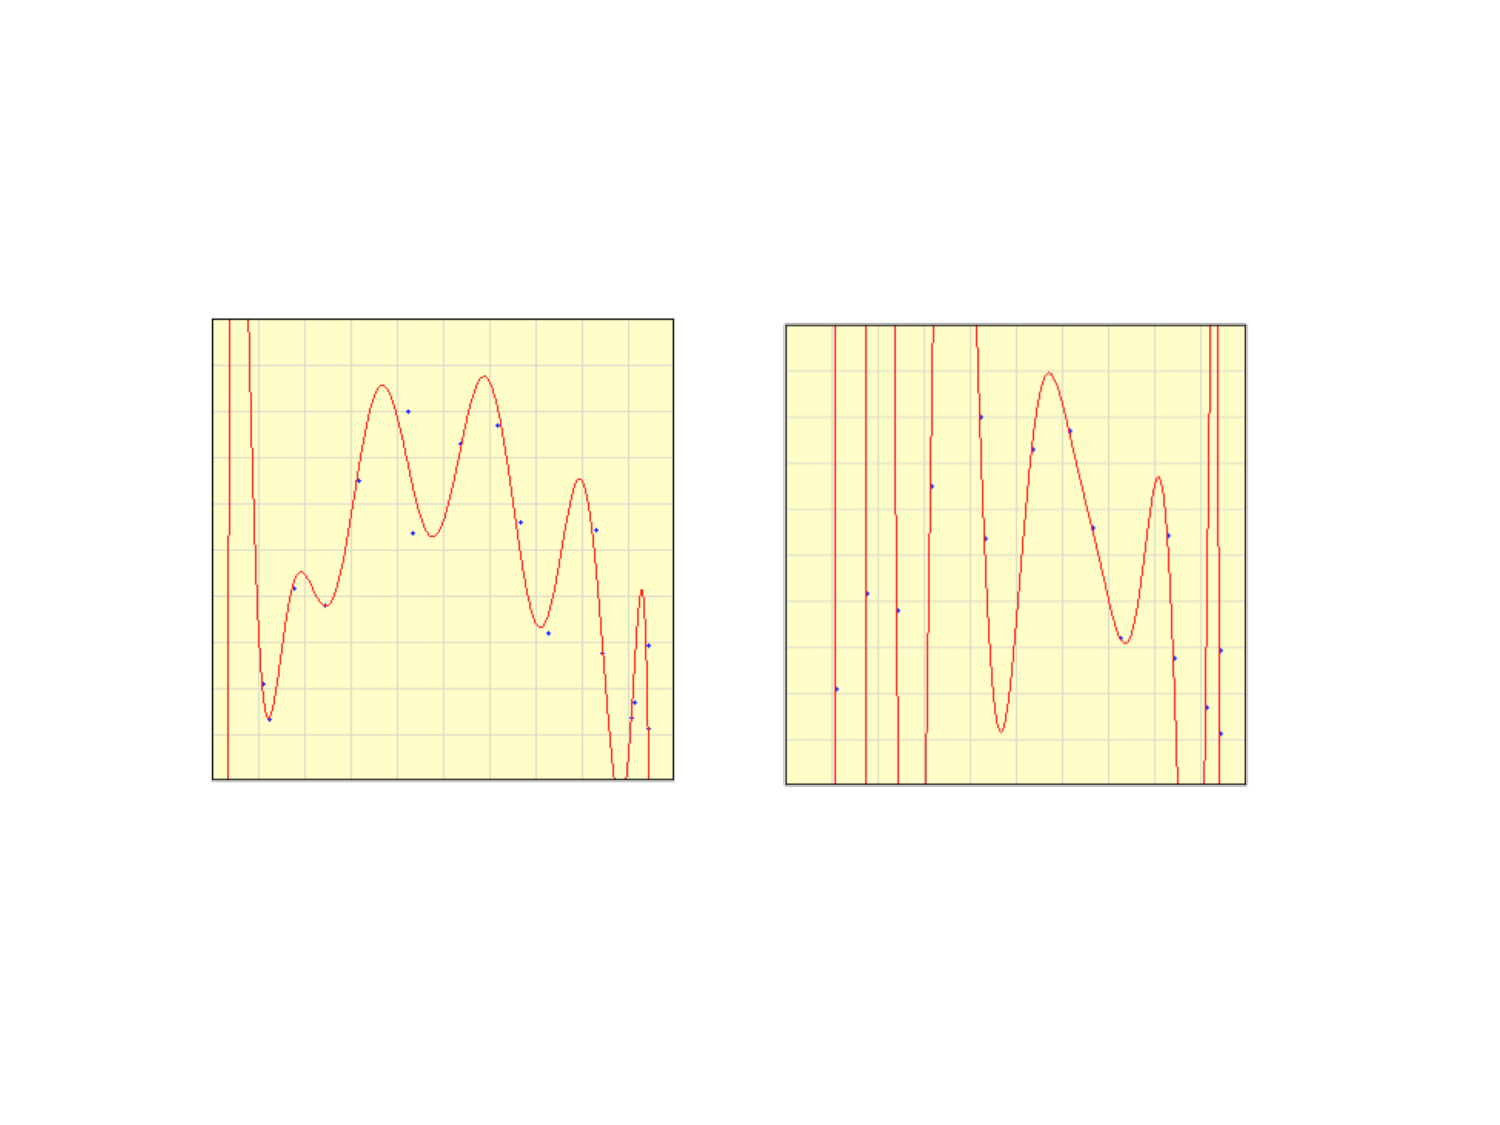
\includegraphics[width=1.2in]{figures/need_to_regularize.pdf}

\subsubsection{Ridge Regression}  \hfill \\
Ridge Regression is the most famous form of linear regression
Here is our old "ordinary" least squares objective function:   \hfill \\
$\displaystyle \widehat{w} = \argmin_w \sum_{j=1}^N [t(x_j) - (w_0 + \sum_{i=1}^k w_i h_i(x_j))]^2$   \hfill \\
It is the same as the previous ones but $i=0$ is pulled out.    \hfill \\
Now for ridge regression, we use that same notation.  \hfill \\
And we add a penalty term that isn't applied to the bias feature:
\begin{align*}
	\widehat{w}_{ridge} &= \argmin_w \sum_{j=1}^N [t(x_j) - (w_0 + \sum_{i=1}^k w_i h_i(x_j))]^2 + \lambda \sum_{i=1}^k w_i^2   \\
	&= \argmin_w (\bm{H}\bm{w} - \bm{t})^T(\bm{H}\bm{w}-\bm{t}) + \lambda \bm{w}^T I_{0+k} \bm{w}
\end{align*}
That $I_{0+k}$ matrix is this: 
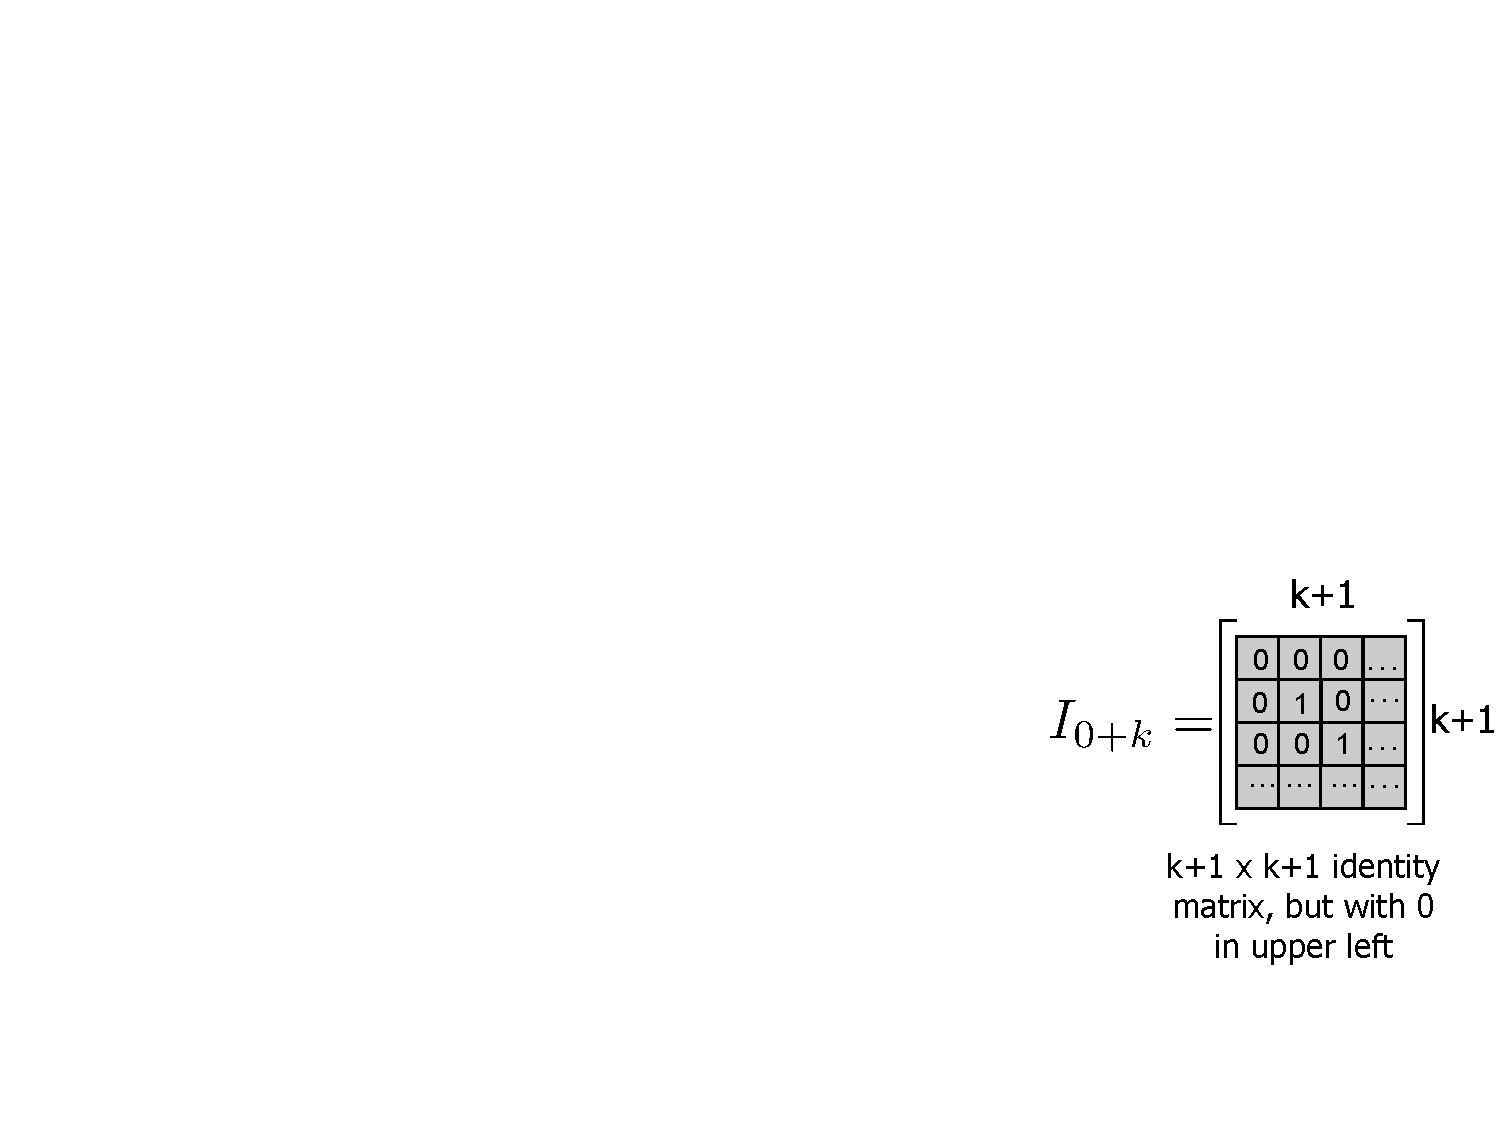
\includegraphics[width=1.0in]{figures/ridge_identity_matrix_with_zero.pdf}  \hfill \\
% Erick hasn't seen this notation.
Allows you to multiply the whole weight array without getting the bias term in there. 

Note: $W^TW$ is $w_i^2$ or $|| w_i ||^2$ 

A similar derivation leads to a closed form solution:  \hfill \\
% http://courses.cs.washington.edu/courses/cse446/16wi/Slides/4_LinearRegression.pdf 
$w_{ridge}^* = (\bm{H}^T\bm{H} + \lambda I_{0+k})^{-1}\bm{H}^T\bm{t}$ \hfill \\
(Recall that un-regularized regression was $w^* = (\bm{H}^T\bm{H})^{-1}\bm{H}^T\bm{t}$).  \hfill \\   \hfill \\

How do you chose how large $\lambda$ is? \hfill \\
* As $\lambda \rightarrow 0$, becomes same as MLE: unregularized.  Large magnitudes of coefficients. \hfill \\
* As $\lambda \rightarrow \infty$, all weights become 0.  \hfill \\   \hfill \\

\subsubsection{Experiment cycle}
\begin{enumerate}
	\item select a hypothesis $f$ to best match the training set.  
		(??) Is this the same as choosing your basis functions (?)
	\item isolate a held-out data set if you have enough data, or do K-fold cross-validation if not enough data. 
	\begin{itemize}
		\item tune hyperparameters ($\lambda$) on the held-out set or via cross-validation.  
			(Try many values of $\lambda$ and chose the best one.) 
		\item You can use the same held-out data set each time if that set is big.  
		\item If doing K-fold, divide the data into k subsets.  
				Repeatedly train on k-1 and test on the remaining one.  
				Average the results. 
		\item find the $w$ that minimizes the error.  
			(Do so by taking the derivative and setting = 0); 
			see ridge regression notes. 
	\end{itemize}
	\item Select basis functions
\end{enumerate}

\subsection{Regularization options: Ridge \& Lasso}  \hfill \\
Ridge: 
\begin{itemize}
	\item $ \displaystyle \widehat{w}_{ridge} = \argmin_w \sum_{j=1}^N [t(x_j) - (w_0 + \sum_{i=1}^k w_i h_i(x_j))]^2 + \lambda \sum_{i=1}^k w_i^2   $ 
	\item $L_2$ penalty.  ("$L_2$ norm of $\bm{w}$).  
		Large distances get penalized more.  $Y = x^2$: 
		don't want errors to cancel each other; differentiable. 
\end{itemize}
Lasso: \hfill \\
\begin{itemize}
	\item$ \displaystyle \widehat{w}_{ridge} = \argmin_w \sum_{j=1}^N [t(x_j) - (w_0 + \sum_{i=1}^k w_i h_i(x_j))]^2 + \lambda \sum_{i=1}^k |w_i|   $ 
	\item L1 penalty: linear penalty pushes more weights to zero.  Allows for a type of feature selection.  But it is not differentiable and there is no closed form solution. 
	\item L1 is absolute value: don't need to square it. 
	\item Lasso may be more useful when you have too many features for the amount of data you get.  
		Example: 100k parameters about companies to predict stock prices but only 100 data points.  
		Could tune lambda until you have about 100 nonzero weights. 
\end{itemize}

Your chose of penalty has huge effects on the algorithm! \hfill \\
Sometimes $L_1$ will do better than $L_2$ and vice versa, but usually $L_2$ is more powerful than $L_1$. \hfill \\
Would be better to use a combination of the penalties than to first reduce the number of features with $L_2$ before applying $L_1$.    \hfill \\
You can generate a lot of basis functions and use $L_1$ to chose the good ones. \hfill \\
\hfill \\

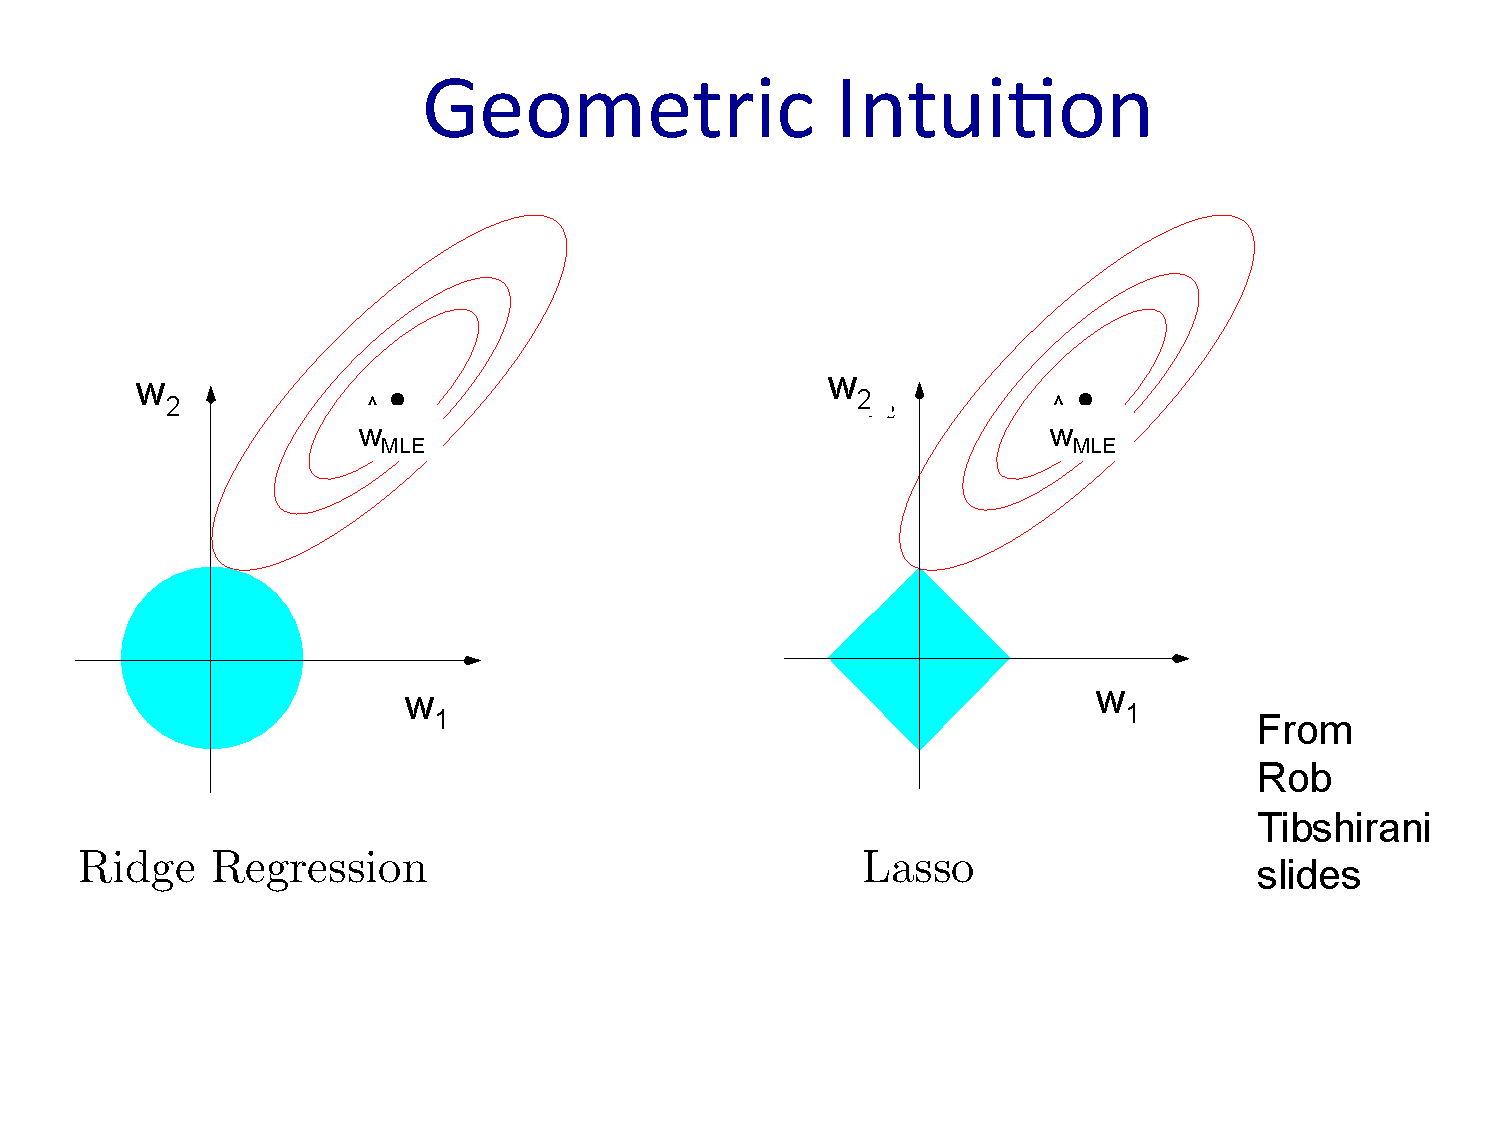
\includegraphics[width=3in]{figures/lasso_and_ridge_geometry.pdf}

This figure shows: 
\begin{itemize}
	\item The contour lines represent the maximum likelihood of the vector of weights.  
		All points on the contour have equal likelihood.
	\item The two axes represent different parameters for two of the weights.  (regression coefficients)
	\item Circles are characteristic of ridge regression (with L2 penalty): Penalty = the magnitude of the vector.
	\item Shapes that are pointy on the axes are characteristic of Lasso (with L1 penalty): the vector components get added. 
	\item Where the likelihood function touches in this $w_1, w_2$ space represents the coefficients of the weights.
		For Ridge Regression, we see that small but nonzero values of the coefficients can be obtained.
		For Lasso Regression, the curves are most likely to touch the diamond on the axes, 
		resulting in coefficients that are truly zero. 
\end{itemize} 

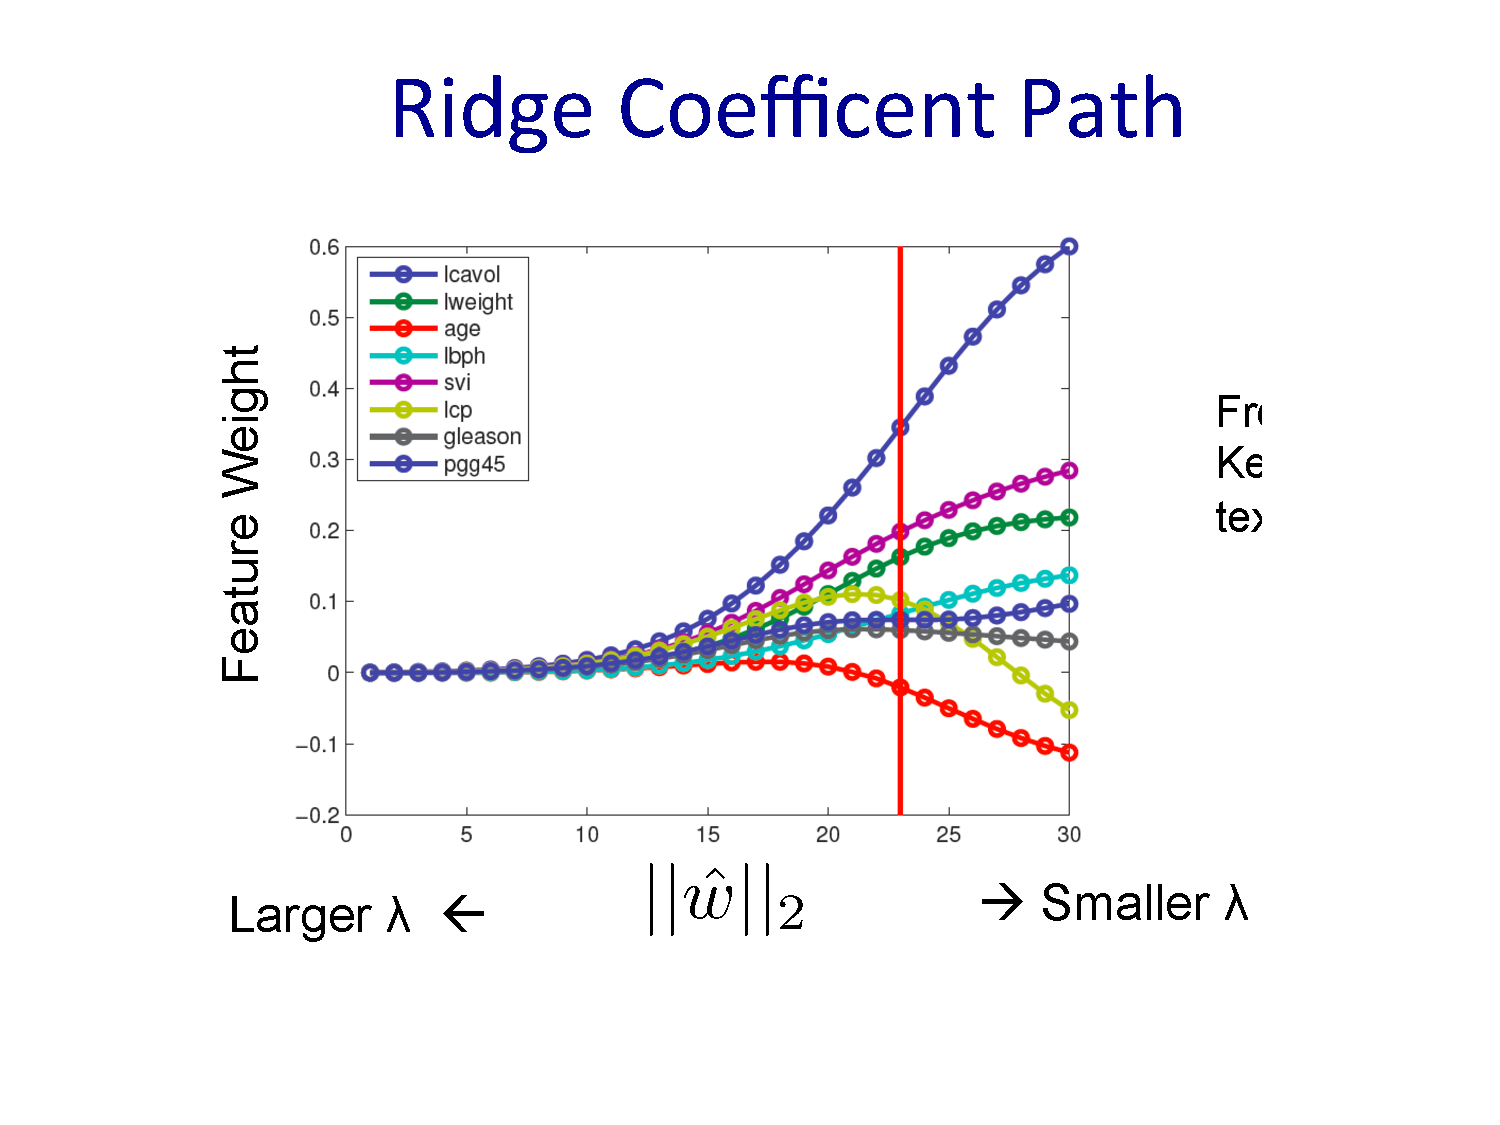
\includegraphics[width=1.8in]{figures/lambda_with_w2.pdf}  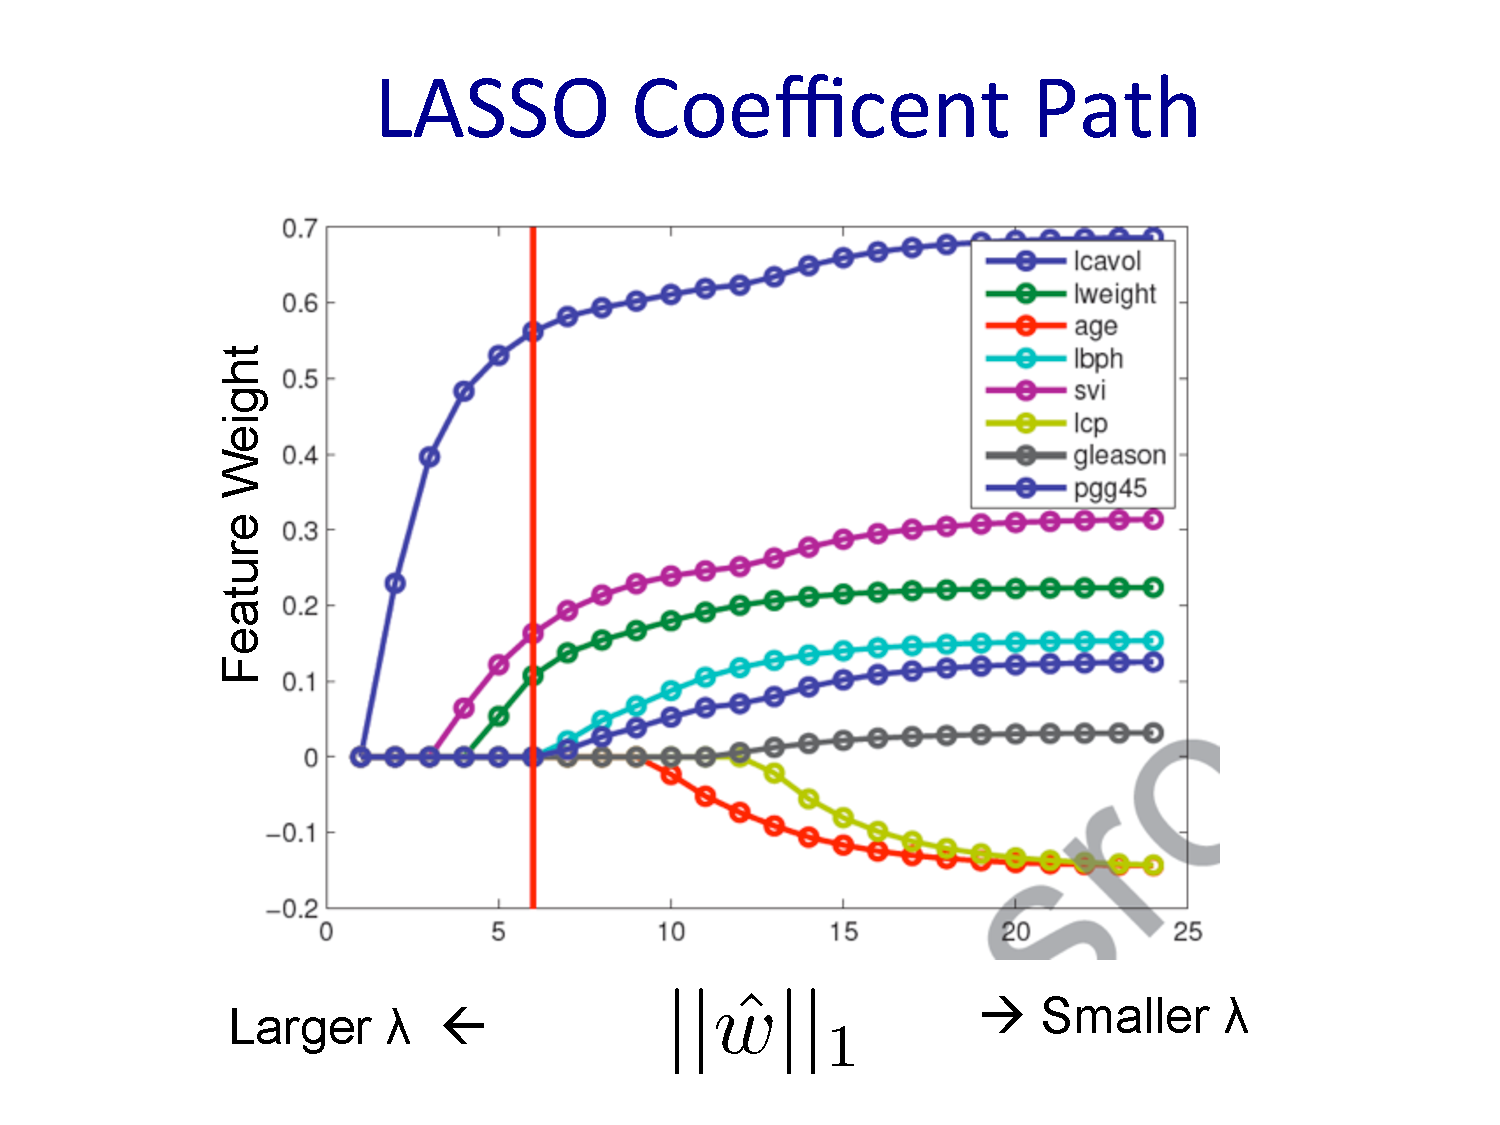
\includegraphics[width=1.6in]{figures/lambda_with_w1.pdf}
Don't compare coefficient magnitudes at given $\lambda$s, 
but do note that for Ridge the gradually come away from the zero axis and in Lasso they are zero until they pop out.   \hfill \\ \hfill \\

\subsection{Bias-Variance Tradeoff}
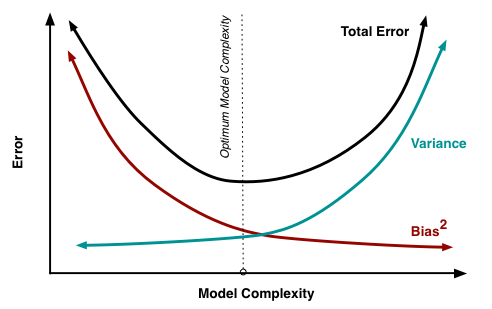
\includegraphics[width=2.0in]{figures/biasvariance.png} 

Your choice of hypothesis class (e.g. degree of polynomial) introduces learning bias.  \hfill \\
The more complex the model, the more the \_\_\_\_ set accuracy goes down  \hfill \\  % had "training" with ?
\textbf{A more complex class } $\rightarrow$ less bias and more variance.   \hfill \\ \hfill \\

From https://www.youtube.com/watch?v=Rm6s6gmLTdg: hfill \\
High bias = inability to represent the true function in the class of functions we are willing to tolerate.
Pulls us to a particular function or class of functions regardless of the data.
Can be from looking only at a specific type of function, or by having strong regularization  \hfill \\
High variance = extremely dependent on the exact data they were trained on.
Might fit the data well, but may do poorly on a different data self.  \hfill \\


From Wikipedia: \hfill \\  % https://en.wikipedia.org/wiki/Bias%E2%80%93variance_tradeoff
Ideally, one wants to choose a model that both accurately captures the regularities in its training data, 
but also generalizes well to unseen data. Unfortunately, it is typically impossible to do both simultaneously. 
High-variance learning methods may be able to represent their training set well, but are at risk of overfitting 
to noisy or unrepresentative training data. 
In contrast, algorithms with high bias typically produce simpler models that don't tend to overfit, 
but may underfit their training data, failing to capture important regularities. \hfill \\  \hfill \\

Models with low bias are usually more complex (e.g. higher-order regression polynomials), 
enabling them to represent the training set more accurately. 
In the process, however, they may also represent a large noise component in the training set, 
making their predictions less accurate - despite their added complexity. 
In contrast, models with higher bias tend to be relatively simple (low-order or even linear regression polynomials), 
but may produce lower variance predictions when applied beyond the training set. \hfill \\ \hfill \\

Adding features (predictors) tends to decrease bias, at the expense of introducing additional variance.   \hfill \\
\hfill \\

Solutions:
\begin{itemize}
	\item Dimensionality reduction and feature selection can decrease variance by simplifying models. 
	\item Similarly, a larger training set tends to decrease variance. 
	\item Use tunable modeling parameters such as applying more significant regularization.
\end{itemize}

\textbf{If held-out is too small, we can end up over-fitting.}


\hfill \\  \hfill \\

\subsection{Error Definitions}

\underline{True ("Prediction") Error}:   \hfill \\
Since the training set error can be a poor measure of the "quality" of the solution, we can use prediction error ("true error").  
The error over all possibilities.   Instead of sum, take expectation. 
\begin{align*}
	error_{true}(\bm{w}) &= E_X[(t(\bm{x_j})-\sum_{i} w_i h_i(\bm{x_j}))^2] \\
		& \mbox{Gold Standard:} \\
	error_{true}(\bm{w}) &= \int_x (t(\bm{x_j})-\sum_{i} w_i h_i(\bm{x_j}))^2 p(\bm{x}) d\bm{x}
\end{align*}
How to get $p(\bm{x})$?  Need to know the true distribution of the data (?).  
You almost never know how to compute p(x).
And, the integral is a very big sum. \hfill \\  \hfill \\

Find $p(x)$ using monte-carlo integration. 
Sample some points, estimate p(x).  
That leads to a fair approximation.  \hfill \\  \hfill \\

The true prediction error is the expectation over \textbf{future} test cases you don't have.  
Since you don't have the x values, you go to probability. 
Pick a point from the distribution, and calculate the \_\_\_\_\_.     \hfill \\  \hfill \\

Sampling approximation of predicted error: \hfill \\
$\displaystyle error_{true}(\bm{w}) \approx \frac{1}{M} \sum_{j=1}^M(t(\bm{x_j} - \sum_i w_i h_i(\bm{x_j}))^2$  \hfill \\
Don't use the training data to predict true error; you've already trained to that data!  You would have too optimistic of a prediction for true error. 

Prediction error is high when the model is too simple \underline{and} too complex, unlike training set error which only penalizes too simple.  \hfill \\
\hfill \\

\underline{Training Set Error}:  \textbf{optimistically biased}  (a.k.a. training error) \hfill \\
$\displaystyle  error_{train}(\bm{w}) = \frac{1}{N_{train}} \sum_{j=1}^{N_{train}}(t(\bm{x_j})-\sum_{i} w_i h_i(\bm{x_j}))^2$ \hfill \\
Decreases exponentially with model complexity.   \hfill \\
\textbf{Training error is a poor prediction of prediction error!} \hfill \\
You expect to see training error to decrease with complexity, but that doesn't mean you have a good solution!  \hfill \\
\hfill \\  \hfill \\
% http://courses.cs.washington.edu/courses/cse446/16wi/Slides/4_LinearRegression.pdf


\underline{Test Error}: (our final measure)  \hfill \\
Uses the same formula as prediction error, except that we have never observed the test data.  See formula below. 
We expect the true error to be smile shaped if the x-axis is model-complexity. 
\hfill \\ \hfill \\

\underline{\textbf{Testing is for the user of your algorithm. }}
The user doesn't care about the values in your model.  They just care about how well it works.  
 They dont' care about the value of your hyperparameters. 


\subsubsection{Effects of $\lambda$ value on model}
% week 4 typed notes. 
 \begin{itemize}
 	\item high lambda $\rightarrow$ simple model $\rightarrow$ lots of zeros $\rightarrow$ high error. 
	\item with lambda = 0 $\rightarrow$ converges ridge regression to regular regression. 
	\item with enough traiing data and lambda = 0, we expect overfitting $\rightarrow$ small training error. 
\end{itemize}

\subsubsection{Choosing $\lambda$}
How to find lambdas? 
\begin{itemize}
	\item try a bunch and find which does best on the held out data set.  
		Can't touch test data, even w/ stick so use held-out set. 
	\item Pick lambda that gives minimum error.
		May not find the bottom-of-the-U shape lambda.  
		But it is ok to be off a bit; the red U might be pretty flat at the bottoms.
\end{itemize}		
This use of the held-out data doesn't count as training.  
Lambda is fixed each time, and we train separately. 
Training on training data, just watching the number on the held-out set. \hfill \\
\textbf{The model's parameters are not determined by the held-out data} \hfill \\
\hfill \\

How do you chose the range of lambda? (practical solution) 
\begin{itemize}
	\item You are limited to a grid search over values of lambda. 
	\item You need a strategy for sweeping that space.   
		Could do a "binary search", or something like a gradient search: 
		take a step until we screw it up, and step back smaller.   
		If it gets worse, you take a smaller step.
	\item From your loss, take the value of your loss (compute it).  \hfill \\
		Loss = $(t(x) - \sum w_i h(x_i))^2$  
        		\textbf{"You should be able to find loss given w}
            	Can compute norm of W, too.  
		If your loss is on the order of 1000 and your norm is on the order of 1, you can use these for defining search space.
                	Firs try lamba = 1, 10, 100, 1000.  
		Find the best from there then explore around there.
		If 100 was good, try 200, etc.   
		You just want to know in which order the loss function is going to appear. 
\end{itemize}

\subsubsection{How to handle error calculations:}
Given a dataset, randomly split it into two parts:  \hfill \\
* training data: $\{ \bm{x_1}, \dots, \bm{x_{N_train}} \}$   \hfill \\
* test data: $\{ \bm{x_1}, \dots, \bm{x_{N_test}} \}$   \hfill \\
Use the training data to optimize parameters $\bm{w}$. \hfill \\
To calculate the test set error, you use the final solution $\bm{w^*}$ and calculate \hfill \\
$\displaystyle error_{test}(\bm{w}) \approx \frac{1}{N_{test}} \sum_{j=1}^{N_{test}} (t(\bm{x_j} - \sum_i w_i h_i(\bm{x_j}))^2$  \hfill \\

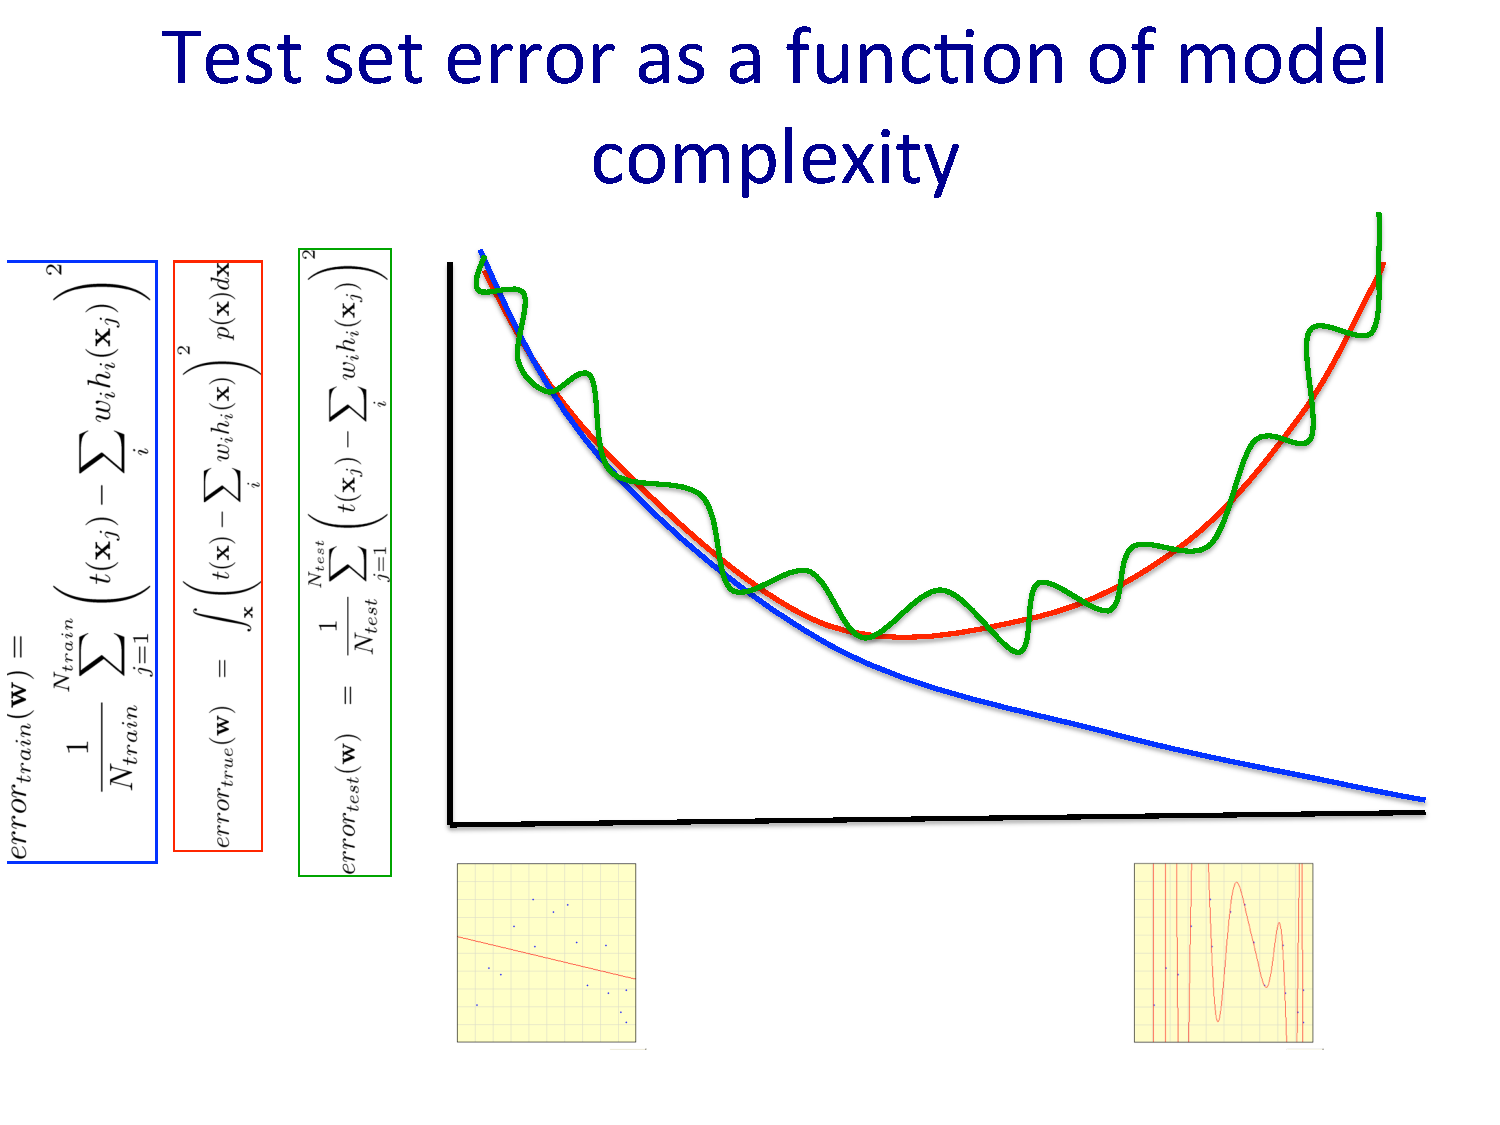
\includegraphics[width=3in]{figures/errors_as_f_of_complexity.pdf}   \hfill \\
(blue is train, red is true, green is test) \hfill \\

\subsubsection{overfitting}
Assume: \hfill \\
* Data generated from distribution D(X,Y). \hfill \\
* A hypothesis space H \hfill \\
Define:  \hfill \\
* Training error: $error_{train}(h)$ \hfill \\
* Data (true) error: $error_{true}(h)$ \hfill \\
We say $h$ \textbf{overfits} the training data if there exists an $h' \in H$ such that:  \hfill \\ 
* $error_{train}(h) < error_{train}(h)'$ and $error_{true}(h) > error_{true}(h)'$

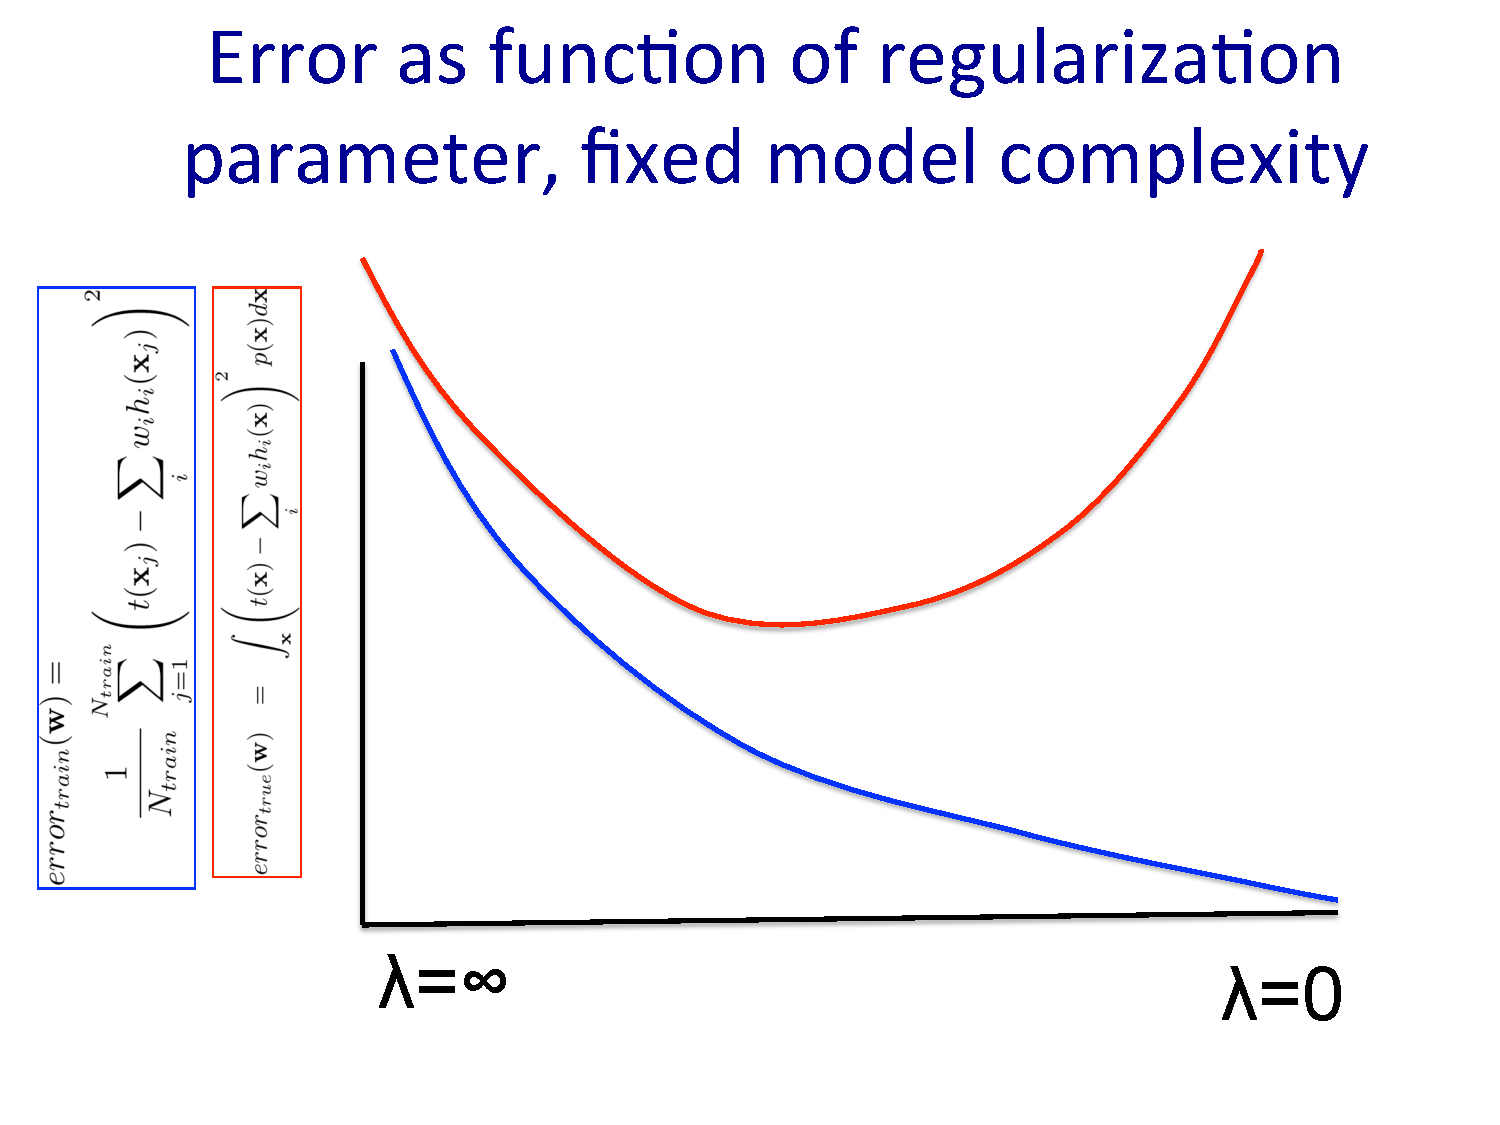
\includegraphics[width=2in]{figures/Error--vs_lambda--fixed_model_complexity.pdf}   \hfill \\
Lambda (the regularization parameter) is fixed.  Blue = training set error.  
Leads to overfitting/too-large-parameters when $\lambda$ --> 0. 
Red = true error, which likes a happy medium $\lambda$.  \hfill \\  \hfill \\

\textbf{Warning}: your test set is only unbiased if you never ever ever do \textbf{any} learning on the data. 
This includes using the test data to select for the degree of the polynomial you fit.   \hfill \\  \hfill \\
(Recall, you can create a held-out/validation set from your training data or do k-fold validation.)  \hfill \\
\hfill \\

The height of the true error (red curve) is the "bias".  \hfill \\

\subsubsection{What you need to know}
Regression:
\begin{itemize}
	\item Basis functions = features
	\item Optimizing a sum of squared errors
	\item Relationship between regression and Gaussians
\end{itemize}
Regularization
\begin{itemize}
	\item Ridge regression math
	\item LASSO formulation
	\item How to set lambda
\end{itemize}
Bias-Variance trade-off





